\section{Implementation}

Groovy was chosen as a language for implementation for two reasons, firstly it has a very efficient web framework called Grails built on the Spring framework, which is not only proven to be very robust and scalable, but is also relatively easy to implement and so enables quick agile development cycles. Previous implementations using Java/Spring and Java/Roo have proved very time-consuming to experiment with, whereas Grails has proven to be more flexible and easier to experiment with. The Groovy language also offers both some functional capability, as well as dynamic meta-programming capability. Domain specific languages (DSL’s) can be easily built on this framework, and this capability offers some scope to build a DSL based on the DataMOF DSL specification and meta-model expanded in the previous section.
 
The Model Catalogue design discussed here has been implemented by building a core Models Catalogue using Groovy within the Grails framework. Prototype implementation was carried out using the EMF/ECore framework, however the Grails framework offered a robust web-based alternative, with enough Model-Driven capability to test out the core ideas expressed here using a maintainable java-based stack that could be worked on by mainstream developers without a detailed knowledge of the Model Driven Engineering. 

The front end user interface was implemented using a combination of HTML with Javascript and CSS, the principal framework used being Angular JS. Communication with the client was carried out using a REST controller, enabling a variety of clients potentially to link up with the Model Catalogue.

GORM was used as a persistence mechanism, with a MySQL relational database as storage, although different GORM adapters made it possible to attach NO SQL datastores such as Neo4J and MongoDB. The full architectural stack is shown in figure\ref{fig:ApplicationArchitectMDR}


\begin{figure}[here]
	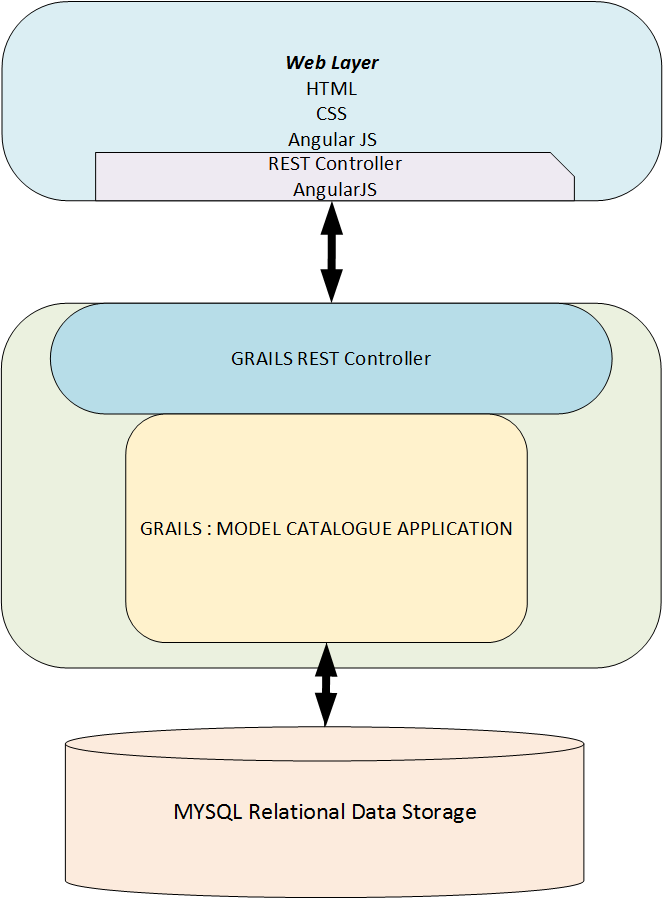
\includegraphics[width=0.5\textwidth,natwidth=610,natheight=642]{ApplicationArchitect1}
	\caption{Overview Architecture} 
	\label{fig:ApplicationArchitectMDR}
\end{figure}

The Grails/GORM framework enabled the Ecore model to generate the basic Grails Domain model, and from that a Groovy DSL was built to handle transformations internally between different representational languages such as XML and excel. A series of importers was built, although due to the simplicity of the DataMOF DSL it was not possible to build exporters for every format. The internal domain model used a basic \emph{Catalogue Element} which was able to link elements via the \emph{relationship} and \emph{relationshipType} classes. Any catalogue element is able to be related to any other catalogue element through a relationship class, this relationship is constrained by the relationshipType object which can prevent different catalogue element types being related, so that a Model cannot directly be related to a say a Datatype Enumeration. 
Relationship types can be added to the Model dynamically, so that even though the relationship between a Model and Datatype enumeration is prevented initially, a new type could be introduced by an administrator or super user to add in that relationship.
Some of the main relationships that are currently modelled in the \emph{Models Catalogue} are as follows:
 
\begin{center}
	\begin{tabular}{ p{1.5cm}  p{1.5cm}  p{1.5cm}   }  % centered columns (5 columns)
		Source & Relationship & Destination  \\
		Model & containment & DataElement   \\
	    Model & containment & Class    \\
	    Model & hierarchical & Model  \\
	    DataElement & supersession & DataElement  \\          
	\end{tabular}
\end{center}

The Core architecture can seen in figure\ref{fig:ApplicationArchitectMDR} 

\begin{figure}[here]
	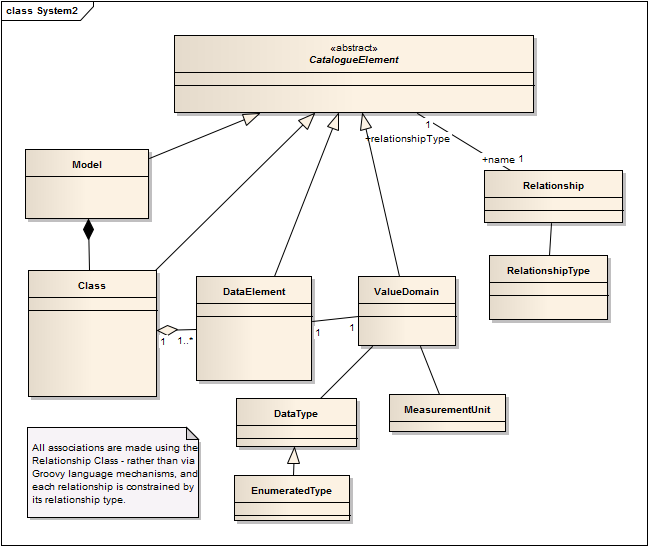
\includegraphics[width=0.5\textwidth,natwidth=610,natheight=642]{System2}
	\caption{Overview Architecture} 
	\label{fig:System2MDR}
\end{figure}
 
\subsection{Modelling Overview}





 
 